\subsection{Entity Component System}

\textit{Entity Component System} (ECS) é um padrão arquitetural baseado no \textit{design} orientado a dados. Ele surgiu na área de desenvolvimento de jogos, onde há uma grande necessidade de otimização e atualizações frequentes no código. Com o passar do tempo, o padrão ECS começou a ser utilizado em outras áreas, como em simulações físicas \cite{flightdynamics}.

O padrão consiste na separação de dado e lógica de tal forma que as vários entidades da aplicação possam ser compostas de dados reutilizáveis e independentes \cite{ecsfaq}, com as funções sendo direcionadas aos dados, e não às entidades em si. Devido ao desacoplamento gerado por essa separação, o padrão ECS garante alta flexibilidade e modularidade, além do aumento de desempenho gerado pela melhor distribuição de dados na memória \cite{ecsstorageinpics}.

Neste projeto, o padrão ECS será um dos principais fundamentos para o \textit{design} e implementação da linguagem de programação, já que o intuito dela será abstrair ele.

\subsubsection{Os Três Elementos Fundamentais do ECS}

Pode-se dizer que o ECS é separado em três elementos fundamentais: entidades, componentes e sistemas \cite{ecsfaq}. Cada um desses elementos desempenha um papel específico na aplicação:

\begin{itemize}
	\item Entidades: identificadores únicos que representam os vários conceitos de uma aplicação. Sozinhas, as entidades não contêm dados nem funcionalidade;
	\item Componentes: estruturas de dados que armazenam informações específicas. Uma entidade pode ter múltiplos componentes diferentes, definindo suas características;
	\item Sistemas: funções responsáveis por processar sobre entidades com um determinado conjunto de componentes — processo denominado \textit{querying}.
\end{itemize}

Como ilustrado na \autoref{fig:diagrama_ecs}, o estado da aplicação é dado por um conjunto de entidades, cada uma com seus respectivos componentes. Os sistemas são responsáveis pela transformação do estado da aplicação, processando as entidades que possuem os componentes necessários para a execução do sistema.

\begin{figure}[H]
	\centering
	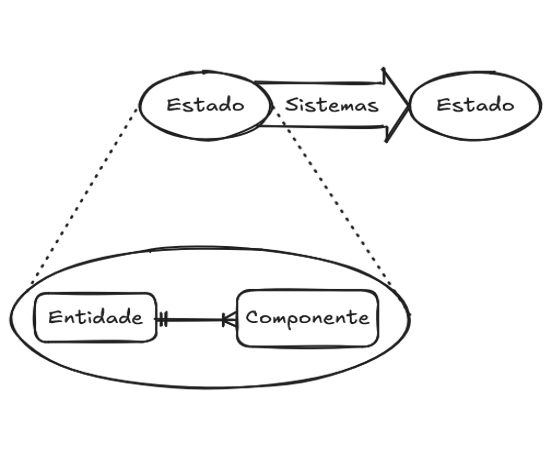
\includegraphics[width=0.35\textheight]{diagrama_ecs}
	\caption{Relação entre entidades, componentes e sistemas.}
	\fonte{Elaboração própria.}
	\label{fig:diagrama_ecs}
\end{figure}

Em termos de código, o padrão ECS pode ser representado sem nenhum construto especializado, mapeando entidades para números únicos, componentes para \textit{structs} e sistemas para funções, como ilustrado no \autoref{cod:exemplo_ecs}.

\codigoRust
\lstinputlisting[
	language=Rust,
	label=cod:exemplo_ecs,
	caption=Implementação simplificada de um padrão ECS incompleto.
]{../codes/exemplo_ecs.rs}
\vspace{-1em}
\fonte{Elaboração própria.}

É importante ressaltar que o \autoref{cod:exemplo_ecs}, por mais que seja funcional e siga o \textit{design} orientado a dados, ainda é uma simplificação da implementação de um padrão ECS incompleto. Na prática, o armazenamento dos dados é feito através de estruturas de dados mais complexas \cite{ecsstorageinpics}, que permitem que entidades escolham quais componentes possuem, que sistemas sejam executados automaticamente, além de outras funcionalidades principais do padrão ECS.

Fora a definição de ECS e seus três elementos fundamentais, o padrão ainda peca pela falta de formalização — quais são as práticas recomendadas ao usar ECS? Como os sistemas são executados? E se apenas entidades, componentes e sistemas não forem suficientes para resolver meu problema? Essas perguntas não possuem respostas definitivas, porém, diferentes autores e implementações abordam o padrão do seu jeito \cite{bevy, flecs}. A seguir, são apresentados alguns conceitos herdados de tais autores e implementações.

\subsubsection{Agendador}

O agendador é um construto com a finalidade de executar todos os sistemas da aplicação, podendo determinar a ordem e frequência de execução de forma declarativa, resolvendo dependência entre sistemas e tornando o ciclo de atualização da aplicação mais previsível \cite{bevy}. Pode-se dizer que, dentre os conceitos mais experimentais, o agendador é o mais próximo de uma formalização.

A \autoref{fig:diagrama_agendador} ilustra o agendador executando os sistemas de forma cíclica e sequencial, onde cada sistema é executado uma vez por ciclo. O agendador pode ser configurado para executar sistemas em diferentes momentos do ciclo, como antes ou depois de outros sistemas.

\begin{figure}[H]
	\centering
	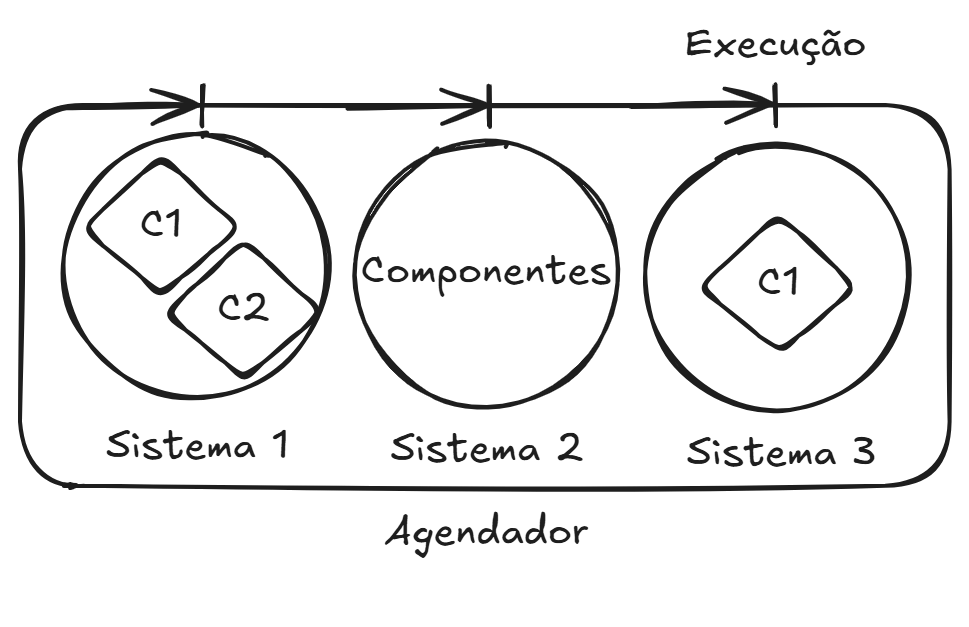
\includegraphics[width=0.3\textheight]{diagrama_agendador}
	\caption{Agendador executando os sistemas de forma cíclica e sequencial.}
	\fonte{Elaboração própria.}
	\label{fig:diagrama_agendador}
\end{figure}

\subsubsection{Relacionamento de Entidades}

Independente da aplicação, é muito comum a necessidade de relacionar diferentes conceitos entre si. Exemplo disso são os sistemas de arquivos, onde pastas podem conter arquivos, uma relação pai-filho.

Relacionamento de entidades (do inglês, \textit{entity relationship}) é um conceito que supre essa necessidade, permitindo que entidades se relacionem entre si. O autor da biblioteca Flecs, \citeonline{flecs}, explica o conceito fazendo uma paralela com o simples ato de adicionar um componente a uma entidade, como ilustrado na \autoref{fig:entidade_posicao}.

\begin{figure}[H]
	\centering
	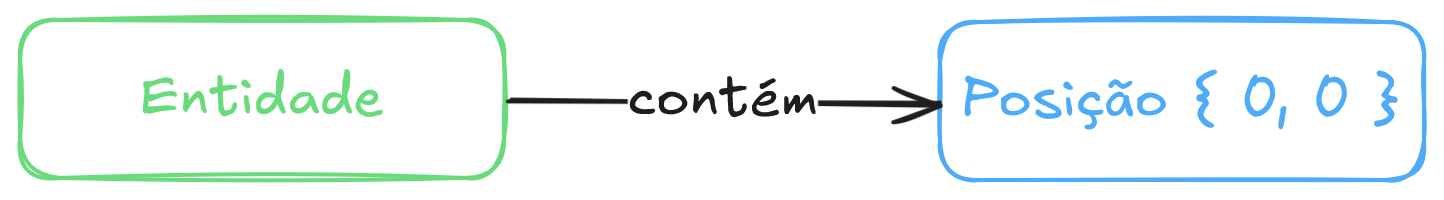
\includegraphics[height=0.06\textheight]{entidade_posicao}
	\caption{Representação do relacionamento entre o Sol, a Terra e a Lua.}
	\fonte{Adaptado de \citeonline{entityrelationships}.}
	\label{fig:entidade_posicao}
\end{figure}

Do mesmo jeito que se adiciona um único componente a uma entidade, como mostra a \autoref{fig:entidade_posicao}, pode-se criar um relacionamento entre duas entidades adicionando uma tupla componente-entidade, onde o componente dita o tipo de relação.

Como exemplo, a \autoref{fig:relacionamento_entidades} ilustra o relacionamento entre o Sol, a Terra e a Lua, onde a Terra é filha do Sol e a Lua é filha da Terra.

\begin{figure}[H]
	\centering
	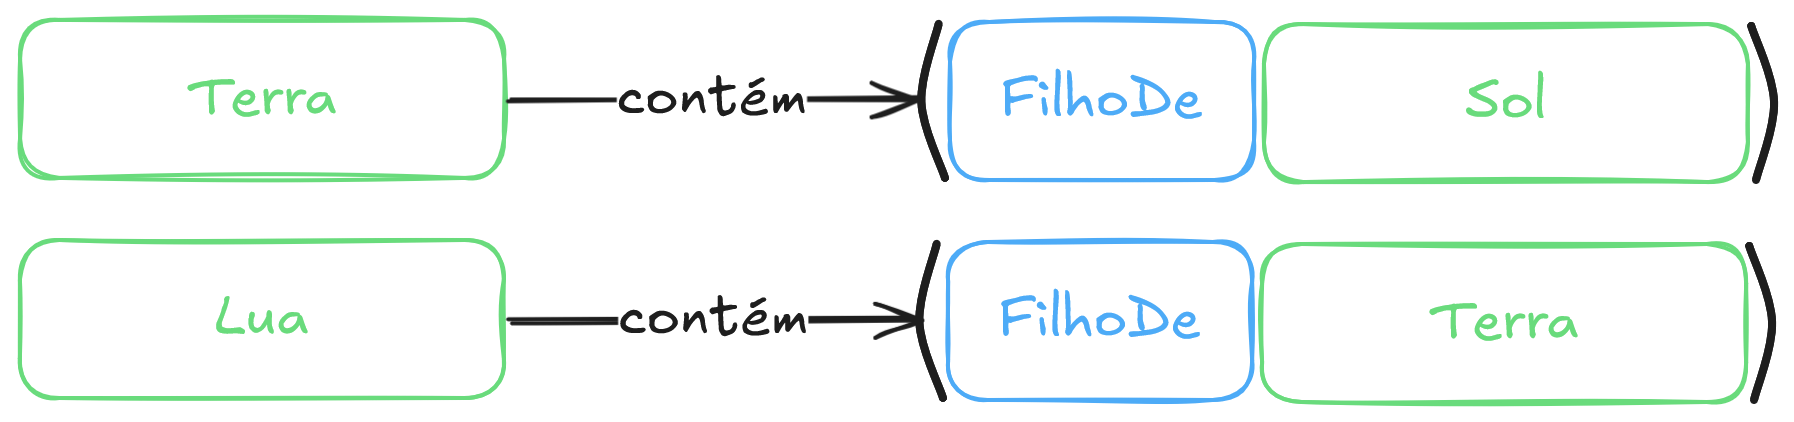
\includegraphics[height=0.13\textheight]{relacionamento_entidades}
	\caption{Representação do relacionamento entre o Sol, a Terra e a Lua.}
	\fonte{Adaptado de \citeonline{entityrelationships}.}
	\label{fig:relacionamento_entidades}
\end{figure}
